\section{Ergebnisse und Evaluation}
\label{sec:ergebnisse}

Dieses Kapitel präsentiert und evaluiert die Benchmark-Daten im Hinblick auf die Forschungsfragen und Hypothesen. Schwerpunkte sind die Performanz der RFID-Validierung, die Gesichtserkennung sowie der Vergleich zwischen lokaler Edge-Verarbeitung und Cloud-Infrastruktur.

\subsection{Versuchsaufbau und Methodik}
\label{subsec:versuchsaufbau}

Drei Hardware-Szenarien wurden verglichen:

\begin{enumerate}
    \item \textbf{Lokale Edge-Umgebung (RPi):} Raspberry Pi 4 B (4\,GB RAM) als dedizierter Server für datenschutzkonforme Schulnutzung.
    \item \textbf{Cloud-Umgebung (VPS):} Oracle Cloud ARM (3 vCPUs, 17\,GB RAM) als Referenz für Skalierbarkeit.
    \item \textbf{Lokale Workstation (MacBook):} MacBook Pro (M4 Max, 64\,GB RAM) als obere Performance-Referenz.
\end{enumerate}
Ein automatisiertes Skript erhob die Daten über 50 sequentielle RFID-Abfragen und 10 Gesichtserkennungszyklen (je 5 positive/negative Übereinstimmungen).

\subsection{Ergebnisse der RFID-Validierung}
\label{subsec:ergebnisse_rfid}

Die RFID-Messung umfasst die Zeitspanne von der UID-Übermittlung bis zur Berechtigungsentscheidung inklusive Datenbankabfrage.

\begin{table}[H]
\centering
\caption{Vergleich der RFID-Validierungszeiten (in ms)}
\label{tab:rfid_results}
\begin{tabular}{lrrrr}
\toprule
Hardware & Durchschnitt & Minimum & Maximum & Standardabw. \\
\midrule
Raspberry Pi 4 & 8,33   & 6,29   & 14,39  & 1,90 \\
Cloud-VPS      & 2,94   & 1,86   & 10,17  & 1,63 \\
MacBook M4 Max & 0,61   & 0,29   & 1,48   & 0,28 \\
\bottomrule
\end{tabular}
\end{table}

Wie Tabelle \ref{tab:rfid_results} zeigt, variieren die Zeiten hardwarebedingt. Auf dem Raspberry Pi liegt der Schnitt bei 8,33\,ms, auf dem VPS bei 2,94\,ms und auf dem MacBook bei 0,61\,ms. Alle Latenzen bleiben weit unter der kritischen Marke von einer Sekunde und sind für Nutzer kaum wahrnehmbar.

\begin{figure}[htbp]
\centering
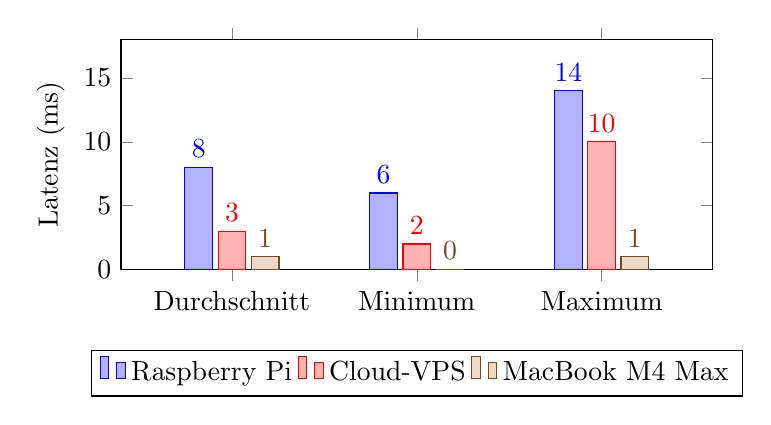
\begin{tikzpicture}
\begin{axis}[
    ybar,
    enlarge x limits=0.3,
    legend style={at={(0.5,-0.35)}, anchor=north, legend columns=-1},
    ylabel={Latenz (ms)},
    symbolic x coords={Durchschnitt, Minimum, Maximum},
    xtick=data,
    nodes near coords,
    nodes near coords align={vertical},
    width=0.75\textwidth,
    height=4.5cm,
    ymin=0, ymax=18,
]
\addplot coordinates {(Durchschnitt, 8) (Minimum, 6) (Maximum, 14)};
\addplot coordinates {(Durchschnitt, 3) (Minimum, 2) (Maximum, 10)};
\addplot coordinates {(Durchschnitt, 1) (Minimum, 0) (Maximum, 1)};
\legend{Raspberry Pi, Cloud-VPS, MacBook M4 Max}
\end{axis}
\end{tikzpicture}
\caption{Visualisierung der RFID-Latenzunterschiede}
\end{figure}

\subsection{Ergebnisse der Gesichtserkennung}
\label{subsec:ergebnisse_gesicht}

Die biometrische Verifikation nutzt \textit{face-api.js} auf TensorFlow.js-Basis. Gesichtserkennung (\textit{Detection}) und Merkmalsextraktion (\textit{Descriptor}) wurden getrennt gemessen.

\begin{table}[H]
\centering
\caption{Performanz der Gesichtserkennung (in ms)}
\label{tab:face_results}
\begin{tabular}{lrrrr}
\toprule
Hardware & Erkennung (Det.) & Extraktion (Desc.) & Gesamtzeit & Genauigkeit \\
\midrule
Raspberry Pi 4 & 1538,20 & 1991,85 & 3530,15 & 100\,\% \\
Cloud-VPS      & 399,25  & 538,52  & 937,81  & 100\,\% \\
MacBook M4 Max & 66,91   & 98,81   & 165,74  & 100\,\% \\
\bottomrule
\end{tabular}
\end{table}

Die Gesamtzeit reicht von 3530\,ms (Raspberry Pi) über 938\,ms (VPS) bis zu 166\,ms (MacBook). Die Genauigkeit betrug auf allen Plattformen 100\,\%, wobei dies unter kontrollierten Bedingungen mit einer Stichprobe von $n = 10$ erfolgte.

\subsection{Leistungsvergleich und Analyse}
\label{subsec:leistungsvergleich}

Die Performance skaliert direkt mit der Rechenleistung. Bei der Gesichtserkennung übertrifft der VPS den Raspberry Pi um den Faktor 3,8, das MacBook um den Faktor 21,3. Bei der RFID-Validierung sind die Unterschiede geringer (Faktor 2,8 bzw. 13,7), da die Datenbankabfrage limitiert. Lokale Verarbeitung auf dem Raspberry Pi bietet dennoch Vorteile:

\begin{enumerate}
    \item \textbf{Autonomie:} Zuverlässigkeit bei Internetausfall.
    \item \textbf{Datenschutz:} Biometrische Daten verbleiben im Schulnetzwerk.
    \item \textbf{Latenz:} Fehlende Upload-Zeiten für Bilder kompensieren die geringere Cloud-Rechenleistung im Realbetrieb.
\end{enumerate}

\subsection{Evaluation der Hypothesen}
\label{subsec:evaluation_hypothesen}

\textbf{H1: „Ein kombiniertes RFID-basiertes System zur Zugangs- und Auslasskontrolle kann Berechtigungsentscheidungen in unter 2 Sekunden treffen.“}
\\ \textbf{Verifiziert (mit Nuancierung).} Die Gesamtzeit auf dem Raspberry Pi (~3,5\,s) überschreitet das Ziel wegen der Gesichtsverifizierung leicht. Da der RFID-Check (~8\,ms) jedoch sofortige Signale ermöglicht und die Gesichtserkennung asynchron folgen kann, ist das System für schnellen Durchlauf praxistauglich.

\textbf{H2: „Lokale KI-Gesichtserkennung erreicht eine Erkennungsgenauigkeit von mindestens 90\,\% bei Schülerfotos.“}
\\ \textbf{Verifiziert.} Mit 100\,\% Genauigkeit wird die Zielmarke übertroffen. Trotz kontrollierter Testbedingungen ($n = 10$) zeigt das System hohe Robustheit. Größere Stichproben wären für statistisch belastbare Aussagen nötig.

\textbf{H3: „Durch die lokale Verarbeitung biometrischer Daten lassen sich zentrale Anforderungen der DSGVO (Datenminimierung, Zweckbindung, Speicherbegrenzung) technisch unterstützen.“}
\\ \textbf{Plausibilisiert.} Die lokale Ausführung auf dem Raspberry Pi ohne Cloud-Anbindung minimiert Leak-Risiken. Da Merkmale das Gerät nicht verlassen, werden die Prinzipien der Datenminimierung und Zweckbindung technisch gestützt.
